\documentclass[12pt]{article}
\usepackage{graphicx}
\usepackage{enumitem}
\usepackage{amsmath}
\usepackage{gvv-book}
\usepackage{gvv}

\title{\textbf{4.5.10}}
\author{\textbf{EE25BTECH11008 - Anirudh M Abhilash}}
\date{September 30, 2025}

\begin{document}

\maketitle

\section*{Question}

Find the equation of the line passing through the point $(1,2,3)$ and parallel to the vector $3\hat{i} + 2\hat{j} - 2\hat{k}$

\section*{Solution}

Let the point $\vec{h}$ and direction vector $\vec{m}$ be  

\[
\vec{h} = \myvec{1 \\ 2 \\ 3}, \quad 
\vec{m} = \myvec{3 \\ 2 \\ -2}.
\]

The vector equation of the line is given by
\[
\vec{x} = \vec{h} + \kappa \vec{m}, \quad \kappa \in \mathbb{R}.
\]

Expanding,  
\begin{align}
\vec{x} &= \myvec{1 \\ 2 \\ 3} + \kappa \myvec{3 \\ 2 \\ -2} \\[2mm]
           &= \myvec{1 + 3\kappa \\ 2 + 2\kappa \\ 3 - 2\kappa}.
\end{align}

Hence the parametric equations of the line are  
\begin{align}
x &= 1 + 3\kappa, \\ 
y &= 2 + 2\kappa, \\ 
z &= 3 - 2\kappa, \quad \kappa \in \mathbb{R}.
\end{align}

\[
\boxed{\frac{x - 1}{3} = \frac{y - 2}{2} = \frac{z - 3}{-2}}
\]

\begin{figure}[H]\centering
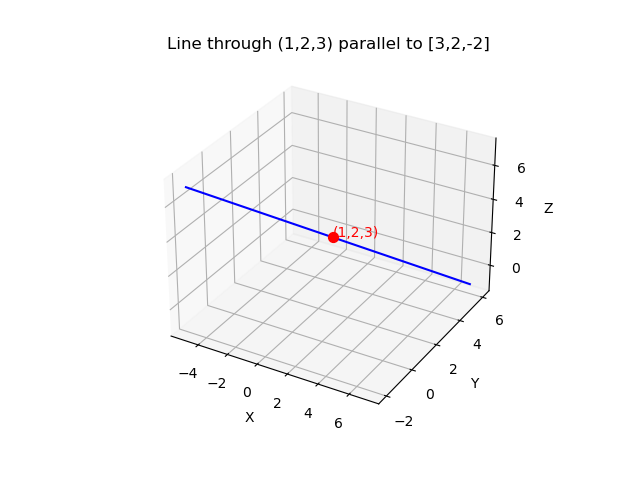
\includegraphics[width=1\columnwidth]{figs/plt.png}
\caption{3D plot of the line}
\label{fig:plt}
\end{figure}

\end{document}
